% ELEC3304 Open Design Project report. Build with: python report/build.py
%
% MARKING CONVENTION (shown in colour until built with --final):
%   \begin{rw}...\end{rw}  BLUE    AI-drafted prose. REWRITE IN YOUR OWN WORDS, then remove the environment.
%   \pend{...}             RED     Number that depends on the pending pole decision (LOGBOOK I-09).
%   \vfy{...}              ORANGE  Something a person must check (source not read, value not verified).
%   Black                          Equations, tables and data: these are the same whoever writes them.
%
% Suggested owners (Aleksei's proposal, 2026-11-02): Controller Design = Aleksei; Numerical Validations = Jack.
\documentclass[conference]{IEEEtran}
\usepackage{cite}
\usepackage{amsmath,amssymb,amsfonts}
\usepackage{graphicx}
\usepackage{xcolor}
\usepackage{textcomp}
\usepackage{url}
% Let wide figures share a page, so they don't queue up at the end of the report.
\renewcommand{\dbltopfraction}{0.95}
\renewcommand{\topfraction}{0.9}
\renewcommand{\textfraction}{0.08}
\renewcommand{\dblfloatpagefraction}{0.8}
\renewcommand{\floatpagefraction}{0.8}
\setcounter{dbltopnumber}{2}
\ifdefined\FIGDIR\graphicspath{{\FIGDIR}}\else\graphicspath{{../figures/}}\fi

\ifdefined\FINAL
  \newenvironment{rw}{}{}
  \newcommand{\pend}[1]{#1}
  \newcommand{\vfy}[1]{}
\else
  \newenvironment{rw}{\color{blue}}{}
  \newcommand{\pend}[1]{{\color{red}#1}}
  \newcommand{\vfy}[1]{{\color{orange}\textbf{[#1]}}}
\fi
\newcommand{\dd}{\dot\theta}
\newcommand{\da}{\dot\alpha}
\newcommand{\figw}{\columnwidth}

\begin{document}

\title{Observer-Based State Feedback for Upright Stabilisation of a Furuta Pendulum}

\author{\IEEEauthorblockN{Jack McCudden}
\IEEEauthorblockA{School of Electrical and Computer Engineering\\
The University of Sydney}
\and
\IEEEauthorblockN{Aleksei \vfy{surname}}
\IEEEauthorblockA{School of Electrical and Computer Engineering\\
The University of Sydney}}

\maketitle

\ifdefined\FINAL\else
\noindent\fbox{\parbox{0.96\columnwidth}{\footnotesize\textbf{Draft key.} {\color{blue}Blue}: AI-drafted prose, rewrite in your own words. {\color{red}Red}: depends on the pending pole decision. {\color{orange}\textbf{[Orange]}}: must be checked by a person. Black: equations, tables, data. Build with \texttt{--final} to remove all marks. \textbf{Results still predate the published damping: refreshed after the next run.}}}
\fi

\begin{abstract}
\begin{rw}
The Furuta pendulum is a small under-actuated laboratory system whose upright position is an unstable equilibrium. Motivated by a serving arm that carries a drink on an unactuated tray joint, this paper tests how far a linear controller can stabilise this highly nonlinear system. A nonlinear model is derived by the Euler--Lagrange method and linearised about upright to give a four-state model with one voltage input and two encoder measurements. Pole placement with integral action on the arm angle is combined with a discrete-time Luenberger observer that estimates the unmeasured velocities at 1\,kHz. The controller is validated on the full nonlinear model with voltage saturation, datasheet-based encoder quantisation, disturbances and parameter uncertainty. It recovers from a \pend{10}\textdegree{} tilt in \pend{0.96}\,s using at most \pend{8.6}\,V and tracks a 30\textdegree{} arm step with \pend{2.0}\% overshoot. Gain margins are \pend{$-4.9$/$+17.8$}\,dB with a phase margin of \pend{38}\textdegree{}. Encoder quantisation causes a small limit cycle, and a firm tap reaches \pend{15.1}\textdegree{}, marginally beyond the 15\textdegree{} limit. Monte Carlo tests show that the observer reduces robustness to parameter error, and that this depends strongly on observer speed.
\end{rw}
\end{abstract}

\begin{IEEEkeywords}
Furuta pendulum, observer-based state feedback, pole placement, linearisation, encoder quantisation
\end{IEEEkeywords}

% =====================================================================
\section{Introduction}
\begin{rw}
Under-actuated systems have more degrees of freedom than control inputs. Spacecraft, underwater vehicles and mobile robots are all examples, and new stabilisation methods are often validated first on simple benchmarks \cite{pujol2014}. The Furuta pendulum, a pendulum free to swing at the tip of a motor-driven horizontal arm, is one such benchmark: it is under-actuated, nonlinear and unstable \cite{hamza2019}, yet small enough to build in a laboratory \cite{antonio2014}. Self-balancing vehicles such as the Segway pose a closely related problem \cite{pujol2014}. So does the \emph{waiter's problem}, in which a robot carries objects on a tray without gripping them while limiting sliding and sloshing \cite{heins2026,biagiotti2023}. Unactuated joints can reduce a manipulator's weight, cost and energy use, and can help fault tolerance \cite{arai1991,araipage}, and a tray with no actuated joint of its own has been shown to reduce sloshing \cite{heins2026}. We use a Furuta pendulum as a scale model of a serving arm that holds a drink on an unactuated joint above the arm.

Control is essential because upright is an unstable equilibrium. In our model a pendulum released just 2\textdegree{} from upright passes 15\textdegree{} in 0.22\,s (Fig.~\ref{fig:openloop}). Holding it there needs continuous feedback, not constant effort: at the exact equilibrium the required voltage is zero, but any deviation grows if left alone.

Models are normally derived by the Euler--Lagrange method \cite{gafvert1998,antonio2014}. Cazzolato and Prime derive the full dynamics with general inertia tensors \cite{cazzolato2011}, and Gäfvert also treats the Coulomb friction seen on real hardware \cite{gafvert1998,gafvert1999}. Hamza et al.\ group the control objectives into swing-up, stabilisation, switching and tracking, and review linear, nonlinear, self-learning and adaptive controllers \cite{hamza2019}. Energy control swings the pendulum up and hands over to a stabilising controller \cite{astrom2000}. Sliding-mode \cite{izutsu2008}, nonlinear predictive \cite{jung2004} and LMI-based H$_\infty$ \cite{pujol2014} methods offer wider operating ranges or designed-in robustness, at the cost of more complex design. For stabilisation near upright, linear methods remain effective: LQR has been verified experimentally on rotary pendulums \cite{tang2020}, and pole placement and LQR were found equivalent on a related reaction-wheel prototype \cite{souza2026}.

Our aim is balance near upright, not swing-up, so a linear state-space design is a suitable choice. It also asks a useful question: how much of a highly nonlinear problem can an LTI approximation solve, and where does it stop working? Because encoders measure only angles, and differentiating them amplifies quantisation \cite{belanger1998}, we use a Luenberger observer \cite{luenberger1964}, and we examine the robustness it costs, since observer-based loops have no guaranteed margins \cite{doyle1978}.

Section~II develops the nonlinear model. Section~III defines the control problem and the linear model. Section~IV designs the controller and observer. Section~V validates them on the nonlinear model, and Section~VI concludes.
\end{rw}
\vfy{Read the sources tagged below before finalising: see docs/10 section 1}

\begin{figure}[t]
\centering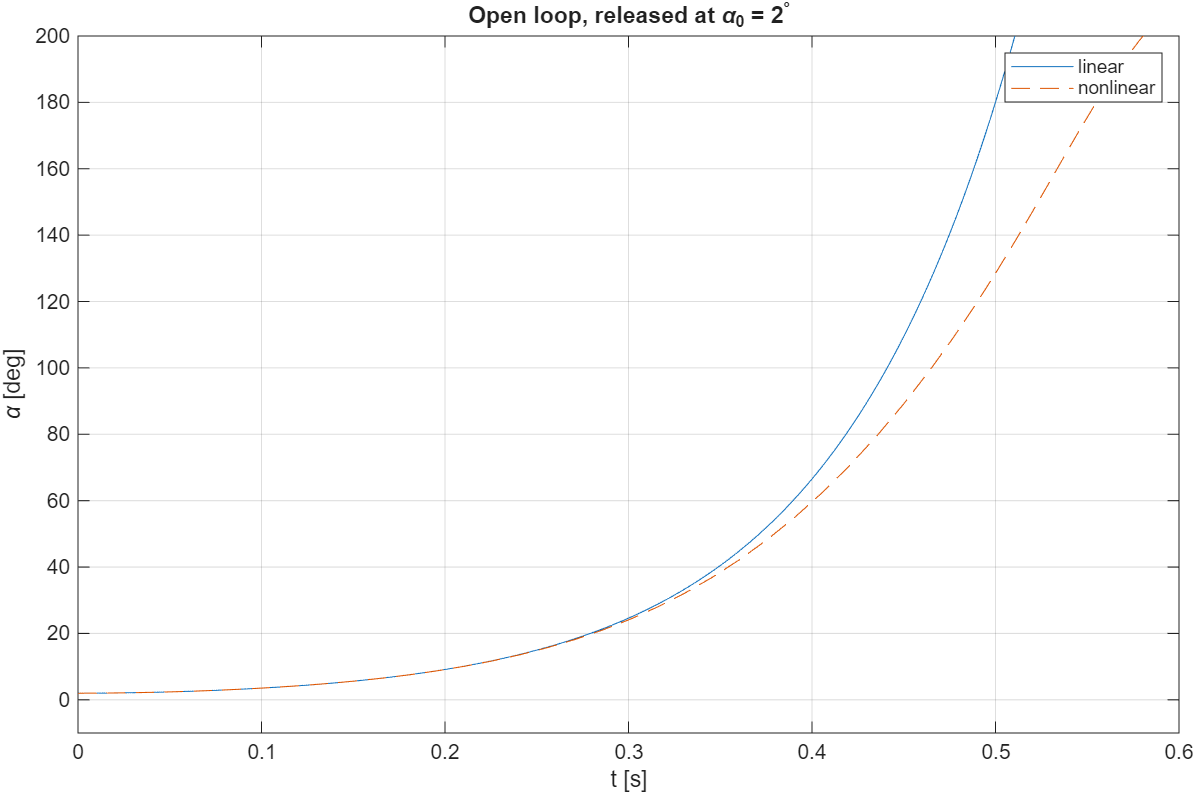
\includegraphics[width=\figw]{w9_openloop_release.png}
\caption{Open-loop release from $\alpha_0=2^\circ$: linear and nonlinear models agree to about 15\textdegree{}, after which the linear model grows without bound while the pendulum falls.}
\label{fig:openloop}
\end{figure}

% =====================================================================
\section{System Model}
\subsection{Nonlinear dynamics}
\begin{rw}
A DC motor rotates a horizontal arm through angle $\theta$. A pendulum swings freely at the arm tip, at angle $\alpha$ from upright, in the plane perpendicular to the arm. Positive $\alpha$ leans against positive arm rotation. We assume rigid links, a uniform slender pendulum, viscous joint friction and negligible motor inductance. Forming the Lagrangian from the kinetic energy of both links and the potential energy $m_p g \tfrac{L_p}{2}\cos\alpha$, and applying the Euler--Lagrange equations \cite{gafvert1998}, gives
\end{rw}
\begin{align}
&\left(J_r + m_p L_r^2 + c\,s_\alpha^2\right)\ddot\theta - \tfrac12 m_p L_p L_r c_\alpha\ddot\alpha \nonumber\\
&\quad + 2c\,s_\alpha c_\alpha\dd\da + \tfrac12 m_p L_p L_r s_\alpha\da^2 = \tau - D_r\dd + \tau_d, \label{eq:arm}\\
&-\tfrac12 m_p L_p L_r c_\alpha\ddot\theta + c\,\ddot\alpha - c\,c_\alpha s_\alpha\dd^2 - \tfrac12 m_p g L_p s_\alpha \nonumber\\
&\quad = -D_p\da + \tau_p, \label{eq:pend}\\
&\tau = \frac{k_m}{R_m}\left(V_m - k_m\dd\right), \label{eq:motor}
\end{align}
\begin{rw}
where $s_\alpha=\sin\alpha$, $c_\alpha=\cos\alpha$, $c=J_p+\tfrac14m_pL_p^2$ is the pendulum's inertia about its pivot, and $\tau_d$, $\tau_p$ are disturbance torques on the arm and pendulum. Equation \eqref{eq:motor} follows from the armature voltage balance with inductance neglected, and shows that back-EMF acts as extra damping on the arm.
\end{rw}

\subsection{Parameters}
\begin{rw}
Table~\ref{tab:params} lists the parameters. Most match a published model of the Quanser QUBE-Servo~2 \cite{xu2023}, and the motor constants match a commercial coreless DC motor \cite{allied}. We model the arm as a uniform bar with the motor at one end, so $J_r=m_rL_r^2/3$, consistent with $L_r$ being the distance from motor axis to pendulum joint and with \cite{gafvert1998}.
\end{rw}
\begin{table}[t]
\caption{Model parameters}\label{tab:params}
\centering\footnotesize\setlength{\tabcolsep}{3pt}
\begin{tabular}{llll}
\hline
Symbol & Meaning & Value & Basis\\ \hline
$R_m$ & Motor resistance & 8.4\,$\Omega$ & \cite{xu2023}\\
$k_m$ & Motor constant & 0.042\,N\,m/A & \cite{xu2023}\\
$m_r$ & Arm mass & 0.095\,kg & \vfy{source}\\
$L_r$ & Motor axis to joint & 0.085\,m & \cite{xu2023}\\
$J_r$ & Arm inertia, $m_rL_r^2/3$ & $2.29\times10^{-4}$\,kg\,m$^2$ & Bar\\
$m_p$ & Pendulum mass & 0.024\,kg & \cite{xu2023}\\
$L_p$ & Pendulum length & 0.129\,m & \cite{xu2023}\\
$J_p$ & About centre, $m_pL_p^2/12$ & $3.33\times10^{-5}$\,kg\,m$^2$ & Rod\\
$D_r$ & Arm damping & 0.0005\,N\,m\,s/rad & \cite{xu2023}\\
$D_p$ & Pendulum damping & 0.0001\,N\,m\,s/rad & \cite{xu2023}\\
$V_{\max}$ & Voltage limit & $\pm10$\,V & Design\\
$q$ & Encoder step & 3.07\,mrad & \cite{heds5540}\\
\hline
\end{tabular}
\end{table}

\subsection{Limitations, uncertainty and disturbances}
\begin{rw}
Real joints also show Coulomb friction and stiction \cite{gafvert1998,gafvert1999}, which we leave out. The arm is not truly a uniform bar, and we ignore its hub, the rotor inertia ($4\times10^{-6}$\,kg\,m$^2$ for the matching motor \cite{allied}, under 2\% of $J_r$) and link flexibility. Parameters are uncertain: damping is hard to measure, and the arm inertia in \cite{xu2023} corresponds to $m_rL_r^2/12$ rather than $/3$. We therefore also test the design on that value, on higher damping, and on $\pm20\%$ random variations of all parameters (Section~V). Taking a glass from the tray changes the payload, so mass uncertainty is part of normal use.

We model three disturbances: a bump to the tray, as a 20\,mN\,m, 20\,ms torque pulse on the pendulum (about a 4.4\,rad/s velocity kick); constant arm drag from the encoder cable, as a 2\,mN\,m step; and random unmodelled torques, as sample-held white noise with assumed standard deviations of 0.2 and 0.05\,mN\,m on the arm and pendulum.
\end{rw}

\subsection{Actuator limits and sensors}
\begin{rw}
We limit the voltage to $\pm10$\,V, a conservative choice inside the $\pm15$\,V drive range of the hardware \cite{quanserdocs} and the 18\,V rating of a motor with matching constants \cite{allied}. That motor is rated at 0.54\,A continuous, with 2.1\,A at stall, so brief currents above the rating are acceptable but sustained ones are not. Its inductance gives an electrical time constant of 0.14\,ms, which justifies neglecting it. The arm angle is limited to about $\pm90^\circ$ by the encoder cable \vfy{assumed}. The controller runs at 1\,kHz, within reach of a low-cost microcontroller: a similar loop has been run on an ESP32 at 1\,ms on a reaction-wheel pendulum \cite{souza2026}.

Only $\theta$ and $\alpha$ are measured, by 512-cycle optical encoders read in quadrature (2048 counts/rev) \cite{heds5540}. The output is digital, so the dominant error is quantisation, not analogue noise:
\end{rw}
\begin{equation}
y_k = q\,\mathrm{round}\!\left(\frac{Cx(kT_s)+b}{q}\right),\quad q=\frac{2\pi}{2048}\text{ rad},\label{eq:quant}
\end{equation}
\begin{rw}
which behaves like noise of standard deviation $\sigma_v=q/\sqrt{12}=0.886$\,mrad while the angle is changing. The datasheet's position error (10\,arcmin typical, 40 maximum) varies slowly with angle, so it is modelled as a constant offset $b$. Velocities are not measured. Differentiating \eqref{eq:quant} is impractical because one count per sample is a 176\textdegree/s jump, which is why an observer is needed.
\end{rw}

% =====================================================================
\section{Problem Definition}
\subsection{Aims and operating point}
\begin{rw}
The aim is to keep the drink upright without spilling, to move the arm to a serving position, and to reject bumps without exceeding actuator limits. The operating point is $\bar x=0$, $\bar u=0$. Any arm angle is also an equilibrium, because $\theta$ does not appear in the dynamics, so $\bar\theta=0$ is chosen without loss of generality. Swing-up is outside the scope.
\end{rw}

\subsection{Linear state-space model}
\begin{rw}
The model is nonlinear and so cannot be used directly with state-space design. We linearise using $\sin\alpha\approx\alpha$, $\cos\alpha\approx1$, and by dropping products of small quantities. With $x=[\theta,\alpha,\dd,\da]^T$, $u=V_m$ and $y=[\theta,\alpha]^T$,
\end{rw}
\begin{equation}
\dot x = Ax+Bu,\quad y=Cx+v,\quad C=\begin{bmatrix}1&0&0&0\\0&1&0&0\end{bmatrix},
\end{equation}
\begin{equation}
A=\begin{bmatrix}0&0&1&0\\0&0&0&1\\0&\frac{bd}{\Delta}&-\frac{cB_{eq}}{\Delta}&-\frac{bD_p}{\Delta}\\0&\frac{ad}{\Delta}&-\frac{bB_{eq}}{\Delta}&-\frac{aD_p}{\Delta}\end{bmatrix},\;
B=\frac{k_m}{R_m\Delta}\begin{bmatrix}0\\0\\c\\b\end{bmatrix},
\end{equation}
\begin{rw}where\end{rw} $a=J_r+m_pL_r^2$, $b=\tfrac12m_pL_pL_r$, $c=J_p+\tfrac14m_pL_p^2$, $d=\tfrac12m_pgL_p$, $\Delta=ac-b^2$, $B_{eq}=D_r+k_m^2/R_m$. \begin{rw}Numerically,\end{rw}
\begin{equation}
A=\begin{bmatrix}0&0&1&0\\0&0&0&1\\0&55.15&-2.61&-0.36\\0&168.58&-2.58&-1.11\end{bmatrix},\;
B=\begin{bmatrix}0\\0\\18.37\\18.16\end{bmatrix}.
\end{equation}
\begin{rw}
The open-loop poles are $0$, $-14.06$, $-1.75$ and $+12.09$\,rad/s, so a lean grows with an 83\,ms time constant. The transfer function from $V_m$ to $\theta$ has a right-half-plane zero at $+10.31$\,rad/s: the arm first moves the wrong way, to tip the pendulum in the direction of travel. This limits how fast the arm can be made to track.
\end{rw}

\subsection{Design criteria}
\begin{rw}
Table~\ref{tab:req} gives the criteria, derived from the serving task using stated assumptions. \emph{Tilt:} for a glass of radius 35\,mm with 10\,mm of freeboard, a level drink spills at $\arctan(10/35)=15.9^\circ$, so we limit $|\alpha|$ to 15\textdegree, where the linear model is also accurate. \emph{Speed:} the first slosh mode of a cylinder satisfies $\omega^2=(1.841g/R)\tanh(1.841H/R)$ \cite{reclari2014}, which is about 22.7\,rad/s. Keeping the dominant poles about five times slower gives $\omega_n\lesssim4.5$\,rad/s, which is close to the limit $z/2\approx5.2$\,rad/s set by the right-half-plane zero. With $\zeta=0.7$ this implies a floor of $T_s\approx1.3$\,s. \emph{Settling:} a commercial robot bar makes over 80 drinks per hour \cite{makrshakr}, or 45\,s per drink. Allowing a quarter of that for settling over four arm moves gives 2.8\,s per move, which we round down to 2.5\,s. Using $\zeta=-\ln(OS)/\sqrt{\pi^2+\ln^2(OS)}$ and $T_s\approx4/(\zeta\omega_n)$, the criteria require $\zeta\ge0.69$ and $\zeta\omega_n\ge1.6$\,rad/s.
\end{rw}

\begin{table}[t]
\caption{Design criteria and results on the nonlinear model}\label{tab:req}
\centering\footnotesize
\begin{tabular}{lll}
\hline
Criterion & Limit & Result\\ \hline
Recovery from 10\textdegree: $|\alpha|<1^\circ$ & $\le1.5$\,s & \pend{0.96\,s}\\
30\textdegree{} step: settling (2\%) & $\le2.5$\,s & \pend{2.40\,s}\\
30\textdegree{} step: overshoot & $\le5$\% & \pend{2.0\%}\\
30\textdegree{} step: undershoot & $\le10$\% & \pend{2.2\%}\\
30\textdegree{} step: rise time & $\ge0.3$\,s & \pend{0.65\,s}\\
Peak voltage (recovery, step, tap) & $\le10$\,V & \pend{9.7\,V}\\
Bump: $\max|\alpha|$ & $\le15^\circ$ & \pend{15.1\textdegree{} (missed)}\\
Bump: $\max|\theta|$ & $\le90^\circ$ & \pend{54.5\textdegree}\\
Arm drag: final $\theta$ error & $<2^\circ$ & \pend{0.22\textdegree}\\
$\pm20$\% parameters: stays upright & all & \pend{36/40 (partial)}\\
\hline
\end{tabular}
\end{table}

% =====================================================================
\section{Controller Design}
\subsection{Reachability and observability}
\begin{rw}
The reachability matrix has rank 4, so all poles can be placed using the single voltage input. The observability matrix has rank 4 with both encoders, and with $\theta$ alone, but only rank 3 with $\alpha$ alone, because the arm angle does not affect the pendulum dynamics. Both encoders are used.
\end{rw}

\subsection{State feedback: an iterative design}
\begin{rw}
The criteria suggest a dominant pair with $\zeta=0.7$, $\omega_n=4$\,rad/s, plus two faster real poles. Matching the coefficients of $\det(sI-A+BK)$ to the desired polynomial gives four linear equations in the gains. Table~\ref{tab:designs} compares three pole sets and an LQR design. D1 places the fast poles further left, but demands 21\,V for a 10\textdegree{} tilt, well beyond the actuator limit, without improving the recoverable angle. We therefore chose D2.

Testing D2 on the nonlinear model exposed a problem: a constant 2\,mN\,m drag leaves the arm 16.7\textdegree{} from its target. We added an integrator $\dot\xi=\theta-r$ with a pole at $-5$. Initially the reference also entered through the proportional term, and a 30\textdegree{} step overshot by 57\%. Feeding the reference only through the integrator (a type-1 servo) reduced this to 2.5\% on the linear model with the same gains. The final law is
\end{rw}
\begin{equation}
u=\mathrm{sat}\!\left(-K_x\hat x-k_i\xi\right),\quad \dot\xi=\theta-r,
\end{equation}
\begin{equation}
K_x=\pend{[-5.04,\;49.09,\;-2.08,\;3.53]},\quad k_i=\pend{-6.87},
\end{equation}
\begin{rw}
with closed-loop poles \pend{$-2.8\pm2.86j$, $-5$, $-12$, $-15$}. The negative arm gains are expected, and follow from the non-minimum-phase behaviour: to move the arm, the controller first tips the pendulum.
\end{rw}

\begin{table}[t]
\caption{Candidate state-feedback designs: $\theta$ step on the linear model, initial voltage at 10\textdegree, and largest recoverable tilt on the nonlinear model}\label{tab:designs}
\centering\footnotesize\setlength{\tabcolsep}{4pt}
\begin{tabular}{lllllll}
\hline
Design & Fast poles & $T_s$ (s) & OS & US & $V_{10^\circ}$ & Max $\alpha_0$\\ \hline
D1 & $-30,-40$ & 1.57 & 5.2\% & 8.8\% & 21.4\,V & 27\textdegree\\
\textbf{D2} & $-12,-15$ & 1.67 & 4.7\% & 4.9\% & 5.7\,V & 28\textdegree\\
D3 ($\omega_n$=3) & $-12,-15$ & 2.17 & 4.7\% & 3.0\% & 5.0\,V & 29\textdegree\\
LQR & (optimal) & 0.97 & 0.8\% & 6.6\% & 7.0\,V & 27\textdegree\\
\hline
\end{tabular}
\end{table}

\subsection{Observer}
\begin{rw}
A discrete-time Luenberger observer runs at $T_s=1$\,ms, using the plant sampled with a zero-order hold and driven by the saturated voltage, so that its estimate stays correct during saturation:
\end{rw}
\begin{equation}
\hat x_{k+1}=A_d\hat x_k+B_du_k+L\left(y_k-C\hat x_k\right).
\end{equation}
\begin{rw}
The estimation error obeys $e_{k+1}=(A_d-LC)e_k$, so it converges to zero if all eigenvalues of $A_d-LC$ lie inside the unit circle. By the separation principle, the closed-loop eigenvalues are those of the controller plus those of the observer, which we confirmed numerically to $3\times10^{-13}$. Table~\ref{tab:obs} shows why the poles were chosen as $-100$, $-110$, $-120$, $-130$\,rad/s ($|z|\le0.905$), which is 6.7--8.7 times the fastest controller pole. Slow observers give smooth estimates, but leave many perturbed plants unstable, consistent with \cite{doyle1978}. Very fast observers amplify quantisation and saturate the motor. A steady-state Kalman filter gives a similar trade-off with modestly less voltage noise (0.14\,V against 0.25\,V RMS for a tap of 16.0\textdegree{} against 15.1\textdegree{}). We kept pole placement, as it was the method taught in this unit.
\end{rw}

\begin{table}[t]
\caption{Effect of observer speed}\label{tab:obs}
\centering\footnotesize\setlength{\tabcolsep}{3pt}
\begin{tabular}{llll}
\hline
Observer poles (rad/s) & RMS $u$ (V) & RMS $\da$ error (\textdegree/s) & Unstable/500\\ \hline
$-15\ldots-18$ & 0.048 & 0.46 & 114\\
$-40\ldots-55$ & 0.098 & 0.83 & 27\\
$\mathbf{-100\ldots-130}$ & 0.244 & 2.79 & 6\\
$-250\ldots-280$ & 0.541 & 7.33 & not run\\
True state (no observer) & -- & -- & 0\\
\hline
\end{tabular}
\end{table}

\subsection{Stability ranges and margins}
\begin{rw}
Table~\ref{tab:ranges} gives the range of each gain over which the sampled linear loop remains stable, with the others held at nominal values. Figure~\ref{fig:margins} shows the loop broken at the plant input. The loop has one unstable open-loop pole, so stability requires it to encircle $-1$ once. The gain can fall to \pend{0.57} times (\pend{$-4.9$}\,dB) or rise to \pend{7.7} times (\pend{$+17.8$}\,dB) nominal before instability. The lower limit exists because an unstable plant needs a minimum gain. The phase margin is \pend{38}\textdegree{} and the delay margin \pend{35}\,ms, far above the 1\,ms sample time. With the true state fed back, the phase margin is \pend{58}\textdegree, so the observer costs about 20\textdegree{}.
\end{rw}

\begin{table}[t]
\caption{Stable range of each parameter, others nominal (*lowest value tested)}\label{tab:ranges}
\centering\footnotesize
\begin{tabular}{llll}
\hline
Gain & Nominal & Stable range & Multiplier\\ \hline
$k_\theta$ & \pend{$-5.04$} & \pend{$-1.44$ to $-11.0$} & \pend{0.29--2.19}\\
$k_\alpha$ & \pend{49.09} & \pend{32.4 to 136} & \pend{0.66--2.78}\\
$k_{\dot\theta}$ & \pend{$-2.08$} & \pend{$-1.39$ to $-3.32$} & \pend{0.67--1.60}\\
$k_{\dot\alpha}$ & \pend{3.53} & \pend{1.83 to 8.08} & \pend{0.52--2.29}\\
$k_i$ & \pend{$-6.87$} & \pend{$-0.14$ to $-19.9$} & \pend{0.02*--2.90}\\
Plant-input gain & 1 & \pend{0.57 to 7.72} & \pend{0.57--7.72}\\
\hline
\end{tabular}
\end{table}

\begin{figure*}[t]
\centering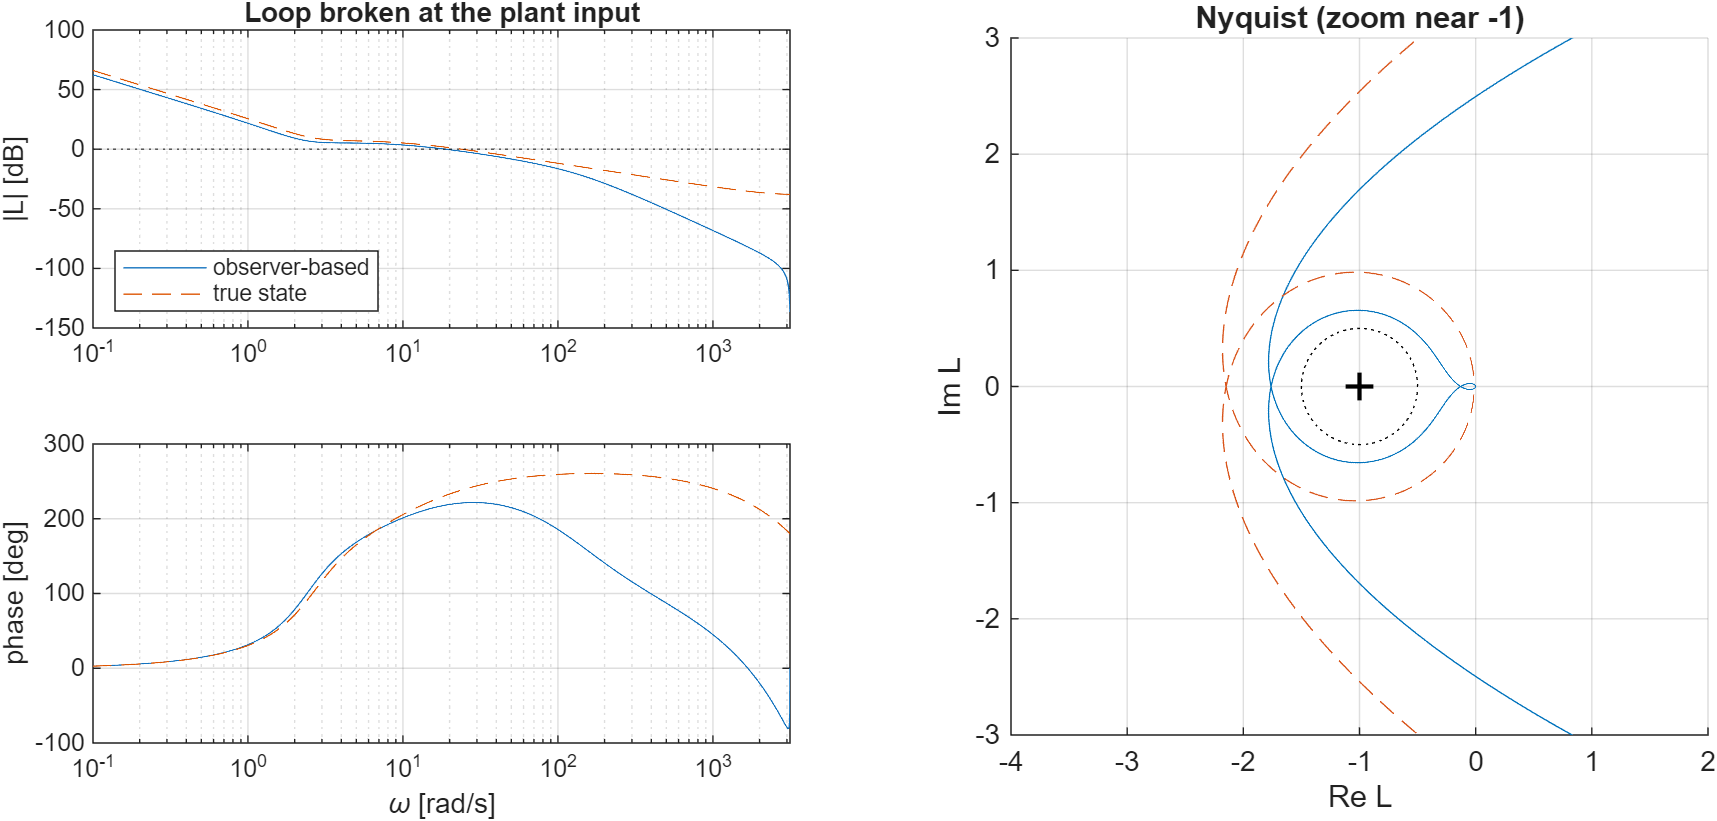
\includegraphics[width=\textwidth]{w12_margins.png}
\caption{Loop broken at the plant input. Left: Bode plot. Right: Nyquist plot near $-1$. Observer-based loop (solid) and true-state loop (dashed).}
\label{fig:margins}
\end{figure*}

% =====================================================================
\section{Numerical Validations}
\begin{rw}
All tests use the nonlinear model \eqref{eq:arm}--\eqref{eq:motor}, integrated with fourth-order Runge--Kutta, with a 1\,kHz controller, zero-order hold, the quantised encoders \eqref{eq:quant} and $\pm10$\,V saturation. Table~\ref{tab:req} summarises the results.
\end{rw}

\subsection{Nominal performance}
\begin{rw}
Figure~\ref{fig:overview} plots three scenarios. Released from 10\textdegree{}, the pendulum is within 1\textdegree{} of upright after \pend{0.96}\,s, with the voltage peaking at \pend{8.6}\,V and a current of \pend{1.02}\,A. The arm swings to \pend{34}\textdegree{} to catch it. The 30\textdegree{} step shows a small initial undershoot, as the right-half-plane zero predicts, and \pend{2.0}\% overshoot, with little voltage.
\end{rw}

\begin{figure*}[t]
\centering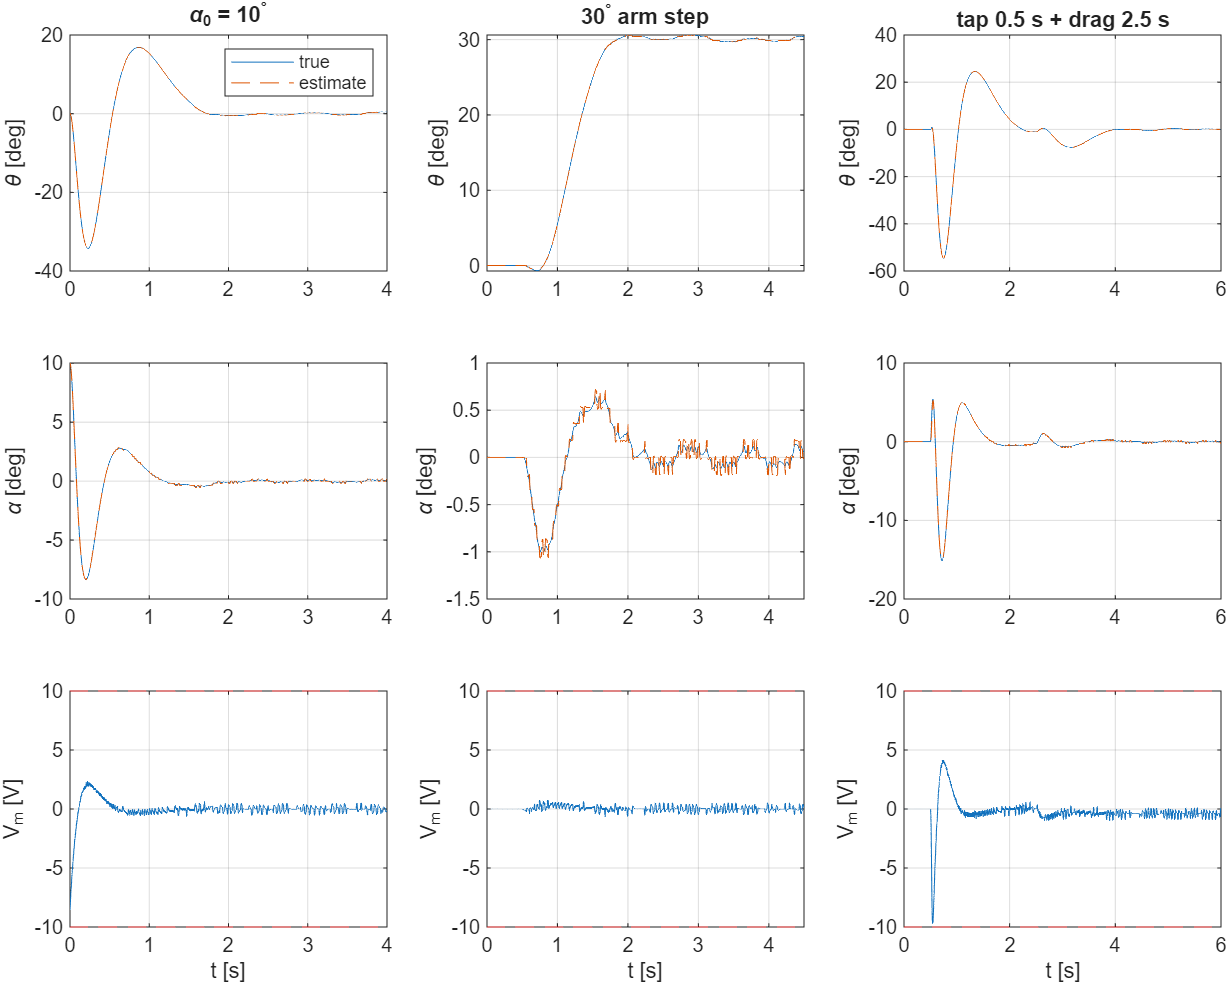
\includegraphics[width=\textwidth]{w12_validation_overview.png}
\caption{Nonlinear closed-loop responses with the observer: release from 10\textdegree{} (left), 30\textdegree{} arm step (centre), tap at 0.5\,s and arm drag from 2.5\,s (right). Rows: arm angle, pendulum angle (true and estimated), motor voltage with limits.}
\label{fig:overview}
\end{figure*}

\subsection{Linear versus nonlinear model}
\begin{rw}
Figure~\ref{fig:linnl} compares the same controller on both models. At 5\textdegree{} and 10\textdegree{} they almost coincide (RMS difference in $\alpha$ of \pend{0.02}\textdegree{} and \pend{0.14}\textdegree{}), so the linear design is valid there. At 20\textdegree{} the linear model demands \pend{17}\,V, which the real motor cannot supply. It saturates at 10\,V, and the arm swings to \pend{83}\textdegree{} rather than \pend{66}\textdegree. The largest recoverable tilt is \pend{22}\textdegree, compared with \pend{28}\textdegree{} for D2 with the true state, so the LTI design solves a useful region of the problem, and that region is limited by saturation and the observer.
\end{rw}

\begin{figure*}[t]
\centering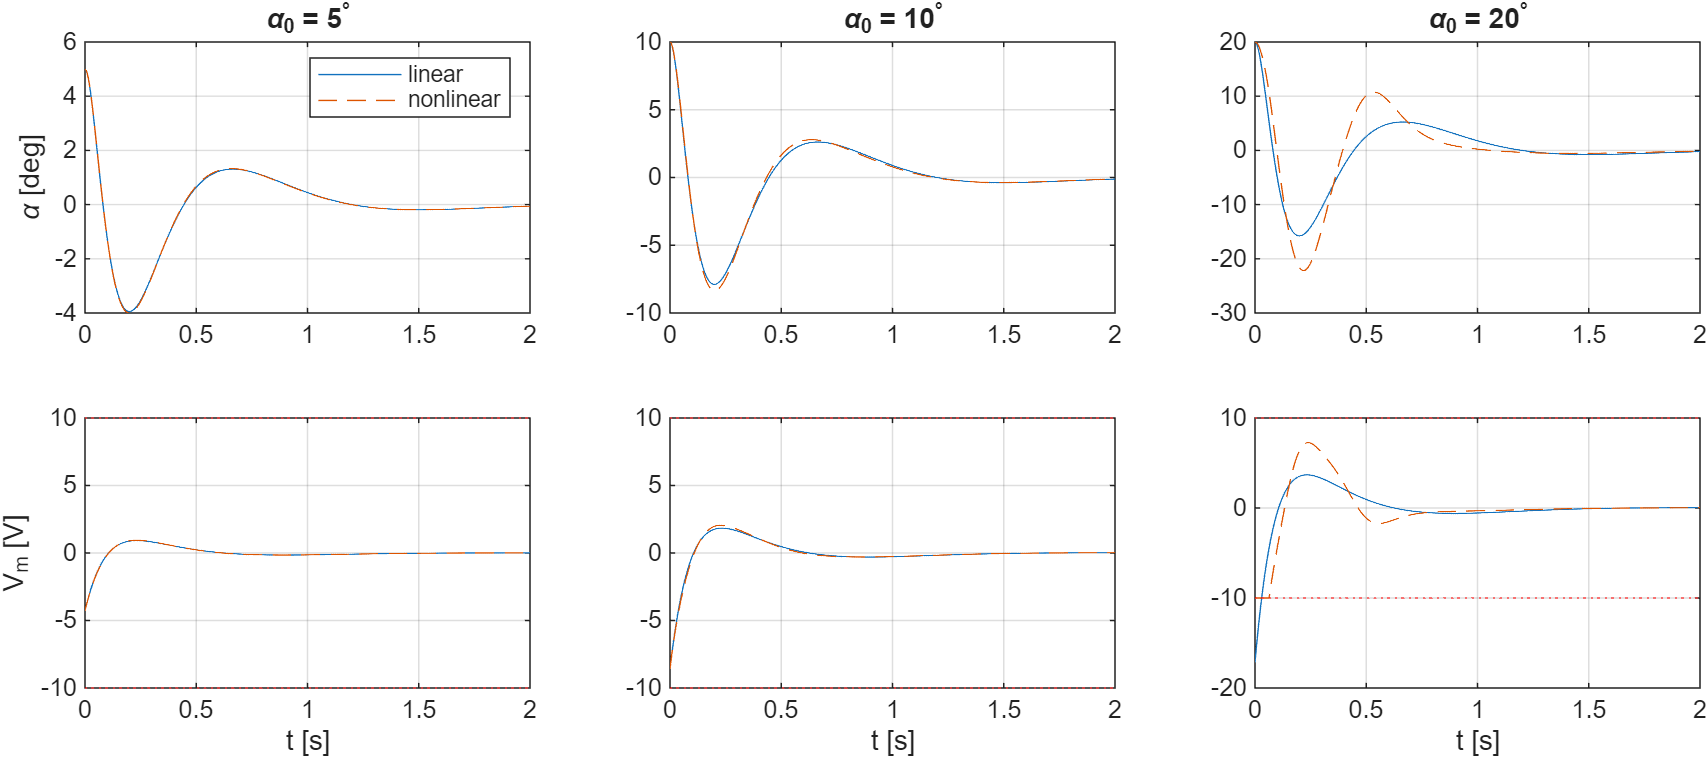
\includegraphics[width=\textwidth]{w12_linear_vs_nonlinear.png}
\caption{Linear and nonlinear responses for releases from 5\textdegree, 10\textdegree{} and 20\textdegree. Voltage limits are dotted.}
\label{fig:linnl}
\end{figure*}

\subsection{Estimation error}
\begin{rw}
Figure~\ref{fig:obs} starts the observer at zero with the pendulum at 10\textdegree. The estimation error falls below 2\% of its initial value within \pend{0.12}\,s, confirming convergence. It does not reach exactly zero, because quantisation sets a noise floor. The large initial error briefly saturates the voltage, which is avoided in practice by initialising $\hat x$ from the first encoder reading.
\end{rw}

\begin{figure*}[t]
\centering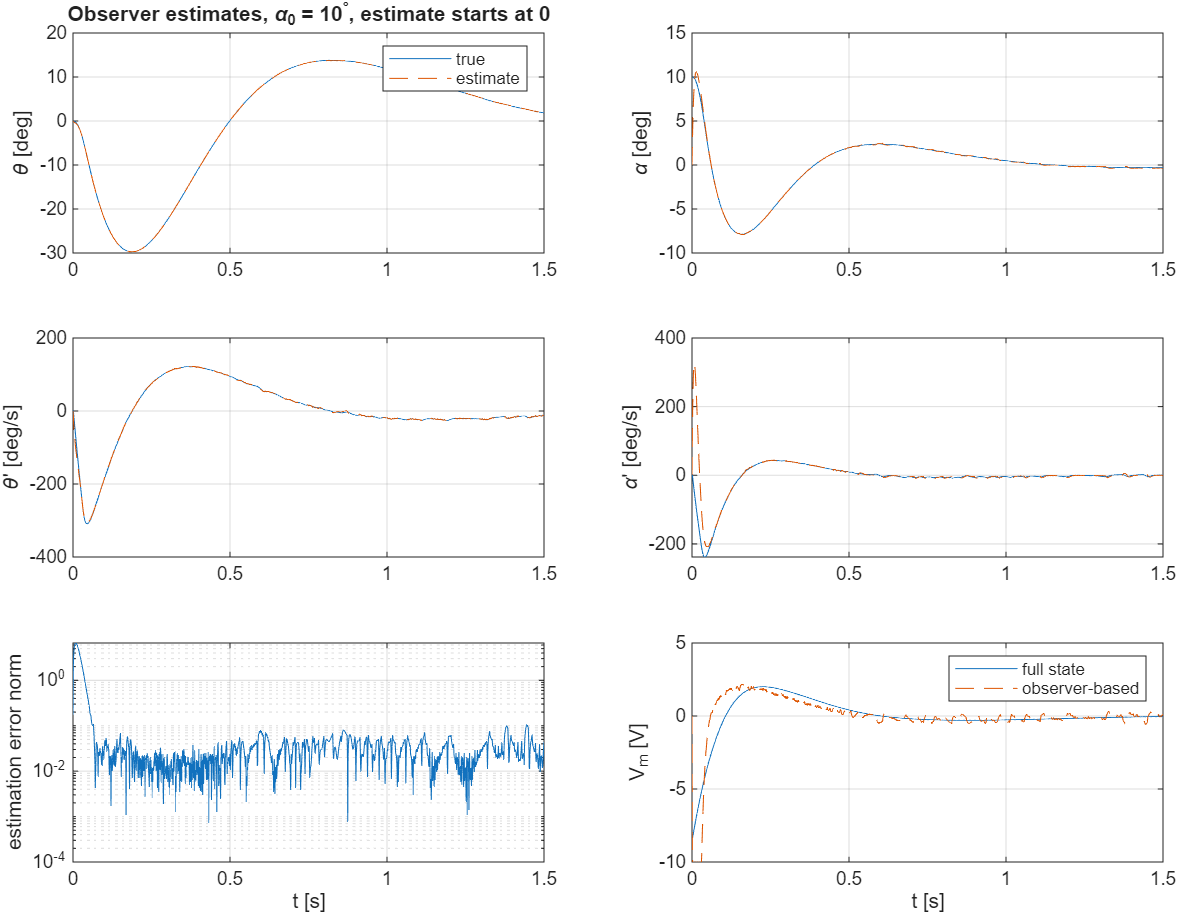
\includegraphics[width=\textwidth]{w11_observer_convergence.png}
\caption{True and estimated states, estimation-error norm (log scale) and voltage, with the estimate starting at zero.}
\label{fig:obs}
\end{figure*}

\subsection{Disturbances and measurement noise}
\begin{rw}
The tap reaches \pend{15.1}\textdegree, missing the 15\textdegree{} criterion by \pend{0.1}\textdegree, with \pend{9.7}\,V and \pend{1.14}\,A, and $|\alpha|$ is below 1\textdegree{} after \pend{0.99}\,s. With the true state the peak is \pend{12.4}\textdegree, so the shortfall is the observer's delay in seeing an unmeasured kick. Under arm drag the integrator leaves \pend{0.22}\textdegree{} of error, against \pend{23}\textdegree{} without it. It also removes encoder offset: for the datasheet's 40\,arcmin maximum, the final error is \pend{0.37}\textdegree, against \pend{19}\textdegree{} without it.

Quantisation has an effect that the linear analysis does not predict. The observer and quantiser form a small limit cycle, with about \pend{1}\textdegree{} peak-to-peak arm ripple and \pend{0.24}\,V RMS. This touches the $\pm0.6$\textdegree{} band of a 30\textdegree{} step, and it raises the measured settling time from \pend{1.81}\,s without quantisation to \pend{2.40}\,s. This voltage noise is feasible, but a slower observer would reduce it at a cost in robustness (Table~\ref{tab:obs}).
\end{rw}

\subsection{Parameter uncertainty}
\begin{rw}
Figure~\ref{fig:mc} shows 40 plants with all parameters randomly varied by $\pm20$\%. All are linearly stable, \pend{36} recover from 10\textdegree{}, and \pend{30} also survive the tap. Over 500 random plants, \pend{6} are linearly unstable with the observer and none with the true state; those failures tend towards a weaker motor than modelled (low $k_m$, high $R_m$). The nominal design also stays stable on the published values: $J_r=m_rL_r^2/12$ (tap \pend{9.5}\textdegree) and damping of 0.0005 and 0.0001 (tap \pend{19.3}\textdegree) \cite{xu2023}. Stability is therefore robust, but the tap response depends strongly on damping, the least certain parameter.
\end{rw}

\begin{figure}[t]
\centering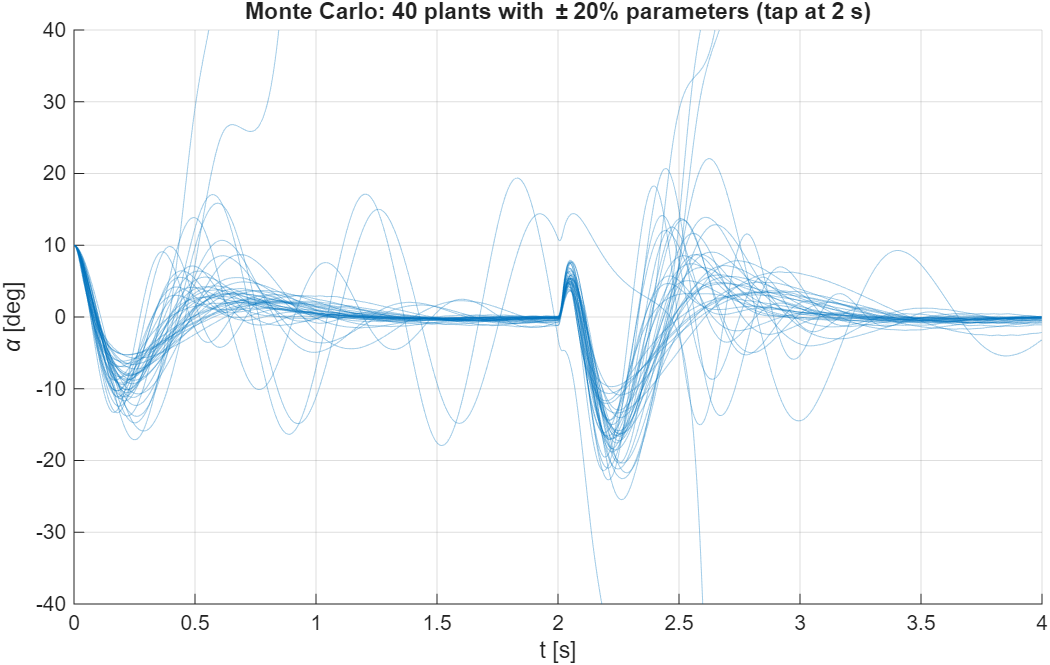
\includegraphics[width=\figw]{w12_monte_carlo.png}
\caption{Pendulum angle for 40 plants with $\pm20$\% random parameters, released from 10\textdegree, with a tap at 2\,s.}
\label{fig:mc}
\end{figure}

% =====================================================================
\section{Conclusions}
\begin{rw}
The Furuta pendulum is a nonlinear, under-actuated benchmark whose upright position requires continuous feedback. We showed that an LTI observer-based controller, designed by pole placement, stabilises the full nonlinear model at 1\,kHz within voltage limits, using only two quantised encoders. It meets all nominal criteria except the tap limit, which it misses by \pend{0.1}\textdegree. Three findings came from testing rather than from the linear design: a double-counted reference that caused 57\% overshoot, the robustness cost of a slow observer, and a quantisation limit cycle.

Future work should measure the damping and arm inertia on real hardware, since these most affect performance. A disturbance-estimating Kalman filter may improve the response to taps, and Coulomb friction should be added to the model. Energy-based swing-up \cite{astrom2000} would extend the controller's operating range to the full circle.
\end{rw}

\section*{Acknowledgment}
\vfy{Declare AI use here, following the Lecture 1 guidelines: check Canvas for the required wording}

\begin{thebibliography}{00}
\bibitem{pujol2014} G. Pujol, L. Acho, A. N\'apoles, and V. P\'erez-Garc\'ia, ``Experimental realization of the Furuta pendulum to emulate the Segway motion,'' arXiv:1405.1834, 2014.
\bibitem{hamza2019} M. F. Hamza, H. J. Yap, I. A. Choudhury, A. I. Isa, A. Y. Zimit, and T. Kumbasar, ``Current development on using Rotary Inverted Pendulum as a benchmark for testing linear and nonlinear control algorithms,'' \textit{Mech. Syst. Signal Process.}, vol. 116, pp. 347--369, 2019. \vfy{abstract only: read}
\bibitem{antonio2014} M. Antonio-Cruz, R. Silva-Ortigoza, C. A. Merlo-Zapata, V. M. Hern\'andez-Guzm\'an, C. M\'arquez-S\'anchez, and J. Sandoval-Guti\'errez, ``Modeling, computer aided design, and construction of a Furuta pendulum test-bed,'' \textit{Res. Comput. Sci.}, vol. 83, pp. 133--144, 2014.
\bibitem{gafvert1998} M. G\"afvert, ``Modelling the Furuta pendulum,'' Dept. Automatic Control, Lund Inst. Technol., Tech. Rep. TFRT-7574, 1998.
\bibitem{cazzolato2011} B. S. Cazzolato and Z. Prime, ``On the dynamics of the Furuta pendulum,'' \textit{J. Control Sci. Eng.}, vol. 2011, Art. no. 528341, 2011. \vfy{not read: open access}
\bibitem{gafvert1999} M. G\"afvert, J. Svensson, and K. J. \AA str\"om, ``Friction and friction compensation in the Furuta pendulum,'' in \textit{Proc. Eur. Control Conf.}, 1999, pp. 3154--3159. \vfy{not read}
\bibitem{astrom2000} K. J. \AA str\"om and K. Furuta, ``Swinging up a pendulum by energy control,'' \textit{Automatica}, vol. 36, no. 2, pp. 287--295, 2000. \vfy{1996 conference version read}
\bibitem{izutsu2008} M. Izutsu, Y. Pan, and K. Furuta, ``Swing-up of Furuta pendulum by nonlinear sliding mode control,'' \textit{SICE J. Control, Meas., Syst. Integr.}, vol. 1, no. 1, pp. 12--17, 2008. \vfy{not read}
\bibitem{jung2004} S. Jung and J. T. Wen, ``Nonlinear model predictive control for the swing-up of a rotary inverted pendulum,'' \textit{J. Dyn. Syst., Meas., Control}, vol. 126, no. 3, pp. 666--673, 2004. \vfy{not read}
\bibitem{tang2020} T. F. Tang, S. H. Chong, and K. K. Pang, ``Stabilisation of a rotary inverted pendulum system with double-PID and LQR control: Experimental verification,'' \textit{Int. J. Autom. Control}, vol. 14, no. 1, 2020. \vfy{not read; add pages}
\bibitem{souza2026} R. H. S. de Souza, J. B. dos Santos, L. D. da Silva, R. Breganon, and U. N. L. T. Alves, ``State-feedback control of a reaction-wheel inverted pendulum prototype,'' \textit{Front. Control Eng.}, vol. 7, Art. no. 1905949, 2026.
\bibitem{belanger1998} P. R. B\'elanger, P. Dobrovolny, A. Helmy, and X. Zhang, ``Estimation of angular velocity and acceleration from shaft-encoder measurements,'' \textit{Int. J. Robot. Res.}, vol. 17, no. 11, pp. 1225--1233, 1998. \vfy{not read}
\bibitem{luenberger1964} D. G. Luenberger, ``Observing the state of a linear system,'' \textit{IEEE Trans. Mil. Electron.}, vol. 8, no. 2, pp. 74--80, 1964. \vfy{not read}
\bibitem{doyle1978} J. C. Doyle, ``Guaranteed margins for LQG regulators,'' \textit{IEEE Trans. Autom. Control}, vol. 23, no. 4, pp. 756--757, 1978.
\bibitem{xu2023} J. Xu, Y. Tan, and X. Chen, ``Robust tracking control for nonlinear systems: Performance optimization via extremum seeking,'' arXiv:2304.00138, 2023.
\bibitem{heins2026} A. Heins and A. P. Schoellig, ``Robotic nonprehensile object transportation with a hanging tray,'' arXiv:2606.10039, 2026. \vfy{abstract only: read}
\bibitem{biagiotti2023} L. Biagiotti, D. Chiaravalli, R. Zanella, and C. Melchiorri, ``Optimal feed-forward control for robotic transportation of solid and liquid materials via nonprehensile grasp,'' arXiv:2306.14212, 2023. \vfy{abstract only: read}
\bibitem{arai1991} H. Arai and S. Tachi, ``Position control of a manipulator with passive joints using dynamic coupling,'' \textit{IEEE Trans. Robot. Autom.}, vol. 7, no. 4, pp. 528--534, 1991. \vfy{abstract only: read}
\bibitem{araipage} H. Arai, ``Control of underactuated manipulators,'' AIST project page. [Online]. Available: \url{https://staff.aist.go.jp/h.arai/uam_e.html}
\bibitem{reclari2014} M. Reclari, M. Dreyer, S. Tissot, D. Obreschkow, F. M. Wurm, and M. Farhat, ``Surface wave dynamics in orbital shaken cylindrical containers,'' \textit{Phys. Fluids}, vol. 26, Art. no. 052104, 2014.
\bibitem{makrshakr} Makr Shakr, ``Toni,'' product page. [Online]. Available: \url{https://www.makrshakr.com/toni}
\bibitem{allied} Allied Motion, ``CL series coreless brushed DC motors,'' data sheet, 2017, CL40 model 16705.
\bibitem{quanserdocs} Quanser, ``QUBE-Servo 2 USB,'' QUARC documentation. [Online]. Available: \url{https://docs.quanser.com/quarc/documentation/qube_servo2_usb.html}
\bibitem{heds5540} Avago Technologies, ``HEDM-55xx/560x \& HEDS-55xx/56xx quick assembly two and three channel optical encoders,'' data sheet AV02-1046EN.
\end{thebibliography}

\end{document}
